\section{RESULTS}\label{sec:results}

Every number in this section comes straight from the campaign's raw telemetry
(Section~\ref{sec:method}); none is hand-typed, so each one traces back to the script that produced
it. \NRunsTotal{} runs finished across the three arms, with zero aborts and zero token-ceiling
breaches. The provenance check turned up $\NProvenanceProblems{}$ deviation across the merged arms:
the campaign's supervisor restarted mid-run after a host infrastructure failure unrelated to the
experiment. The fix that shipped with that restart touched only the supervisor's own health check,
none of the code on a run's execution path, which we confirmed by diff before treating the arms as
one dataset. The first three subsections answer RQ1--RQ3 with the live model, and
Section~\ref{sec:livemock} then shows that those answers hinge on whether the model was real (RQ4).

\subsection{Does the Full Agent System Beat Static Orchestration?}

\begin{table*}[t]
\centering
\caption{Medians [IQR] per configuration, $n$ replicates pooled across scenarios.}
\label{tab:main}
\small
\begin{tabular}{llrrrrr}
\toprule
config & LLM & $n$ & MTTR (s) & cost & manual interv. & decision correct \\
\midrule
baseline & none & 80 & 378 [244] & 158 [113] & 1.00 [0] & 0 [0] \\
rule\_based & none & 80 & 30.0 [15.9] & 158 [113] & 0 [0.250] & 0 [0] \\
autoscale & none & 80 & 52.4 [359] & 82.5 [122] & 0.500 [1.00] & 0 [0] \\
monitor\_only & live & 40 & 359 [210] & 1{,}223 [525] & 1.00 [1.00] & 0 [0] \\
recovery\_only & live & 40 & 220 [75.0] & 1{,}223 [630] & 6.00 [1.00] & 0 [0] \\
optimization\_only & live & 40 & 267 [360] & 76.5 [128] & 1.00 [1.00] & 0 [0.250] \\
schema\_only & live & 40 & 315 [353] & 920 [122] & 1.00 [1.25] & 0 [0.250] \\
full & live & 80 & 235 [143] & 69.8 [35.1] & 6.00 [8.00] & 0 [1.00] \\
\bottomrule
\end{tabular}

\end{table*}

\begin{table*}[t]
\centering
\caption{Effect of each configuration against \texttt{baseline}: bootstrap 95\% CI on the median
  difference, Cliff's $\delta$ with its own 95\% CI, and the Holm-corrected Mann--Whitney $p$-value
  ($^{*}p_{\mathrm{Holm}}<0.05$).}
\label{tab:effects}
\scriptsize
\begin{tabular}{llrrr}
\toprule
config & metric & $\Delta$ median [95\% CI] & Cliff's $\delta$ [95\% CI] & $p_{\mathrm{Holm}}$ \\
\midrule
rule\_based & MTTR (s) & \ensuremath{-}348 [\ensuremath{-}419, \ensuremath{-}303] & \ensuremath{-}0.73 [\ensuremath{-}0.85, \ensuremath{-}0.60] & <0.001$^{*}$ \\
autoscale & MTTR (s) & \ensuremath{-}326 [\ensuremath{-}406, \ensuremath{-}82.7] & \ensuremath{-}0.49 [\ensuremath{-}0.63, \ensuremath{-}0.32] & <0.001$^{*}$ \\
monitor\_only & MTTR (s) & \ensuremath{-}19.2 [\ensuremath{-}99.6, 59.8] & \ensuremath{-}0.09 [\ensuremath{-}0.32, 0.13] & 1.000 \\
recovery\_only & MTTR (s) & \ensuremath{-}159 [\ensuremath{-}229, \ensuremath{-}105] & \ensuremath{-}0.70 [\ensuremath{-}0.83, \ensuremath{-}0.55] & <0.001$^{*}$ \\
optimization\_only & MTTR (s) & \ensuremath{-}111 [\ensuremath{-}188, 15.9] & \ensuremath{-}0.27 [\ensuremath{-}0.50, \ensuremath{-}0.025] & 0.134 \\
schema\_only & MTTR (s) & \ensuremath{-}63.1 [\ensuremath{-}182, 87.4] & \ensuremath{-}0.19 [\ensuremath{-}0.42, 0.056] & 0.638 \\
full & MTTR (s) & \ensuremath{-}143 [\ensuremath{-}212, \ensuremath{-}94.7] & \ensuremath{-}0.56 [\ensuremath{-}0.70, \ensuremath{-}0.42] & <0.001$^{*}$ \\
rule\_based & cost (units) & 0 [0, 0] & 0.00 [\ensuremath{-}0.14, 0.14] & 1.000 \\
autoscale & cost (units) & \ensuremath{-}75.0 [\ensuremath{-}75.0, \ensuremath{-}75.0] & \ensuremath{-}0.62 [\ensuremath{-}0.76, \ensuremath{-}0.45] & <0.001$^{*}$ \\
monitor\_only & cost (units) & 1{,}065 [1{,}065, 1{,}074] & 1.00 [1.0, 1.0] & <0.001$^{*}$ \\
recovery\_only & cost (units) & 1{,}065 [1{,}065, 1{,}389] & 1.00 [1.0, 1.0] & <0.001$^{*}$ \\
optimization\_only & cost (units) & \ensuremath{-}81.0 [\ensuremath{-}81.0, \ensuremath{-}48.3] & \ensuremath{-}0.47 [\ensuremath{-}0.72, \ensuremath{-}0.20] & <0.001$^{*}$ \\
schema\_only & cost (units) & 763 [750, 763] & 1.00 [1.0, 1.0] & <0.001$^{*}$ \\
full & cost (units) & \ensuremath{-}87.7 [\ensuremath{-}96.2, \ensuremath{-}87.7] & \ensuremath{-}0.66 [\ensuremath{-}0.81, \ensuremath{-}0.51] & <0.001$^{*}$ \\
rule\_based & manual interv. & \ensuremath{-}1.00 [\ensuremath{-}1.00, \ensuremath{-}1.00] & \ensuremath{-}0.75 [\ensuremath{-}0.85, \ensuremath{-}0.65] & <0.001$^{*}$ \\
autoscale & manual interv. & \ensuremath{-}0.500 [\ensuremath{-}1.00, 0] & \ensuremath{-}0.50 [\ensuremath{-}0.61, \ensuremath{-}0.39] & <0.001$^{*}$ \\
monitor\_only & manual interv. & 0 [0, 0] & 0.28 [0.15, 0.42] & <0.001$^{*}$ \\
recovery\_only & manual interv. & 5.00 [5.00, 5.50] & 0.97 [0.93, 1.0] & <0.001$^{*}$ \\
optimization\_only & manual interv. & 0 [0, 1.00] & 0.20 [\ensuremath{-}0.050, 0.42] & 0.121 \\
schema\_only & manual interv. & 0 [0, 0] & 0.25 [0.12, 0.38] & <0.001$^{*}$ \\
full & manual interv. & 5.00 [5.00, 8.00] & 0.79 [0.70, 0.88] & <0.001$^{*}$ \\
rule\_based & decision correct & 0 [0, 0] & 0.00 [0, 0] & 1.000 \\
autoscale & decision correct & 0 [0, 0] & 0.00 [0, 0] & 1.000 \\
monitor\_only & decision correct & 0 [0, 0] & 0.00 [0, 0] & 1.000 \\
recovery\_only & decision correct & 0 [0, 0] & 0.00 [0, 0] & 1.000 \\
optimization\_only & decision correct & 0 [0, 0] & 0.25 [0.12, 0.38] & <0.001$^{*}$ \\
schema\_only & decision correct & 0 [0, 0] & 0.25 [0.12, 0.38] & <0.001$^{*}$ \\
full & decision correct & 0 [0, 1.00] & 0.42 [0.31, 0.54] & <0.001$^{*}$ \\
\bottomrule
\end{tabular}

\end{table*}

\begin{figure*}[t]
\centering
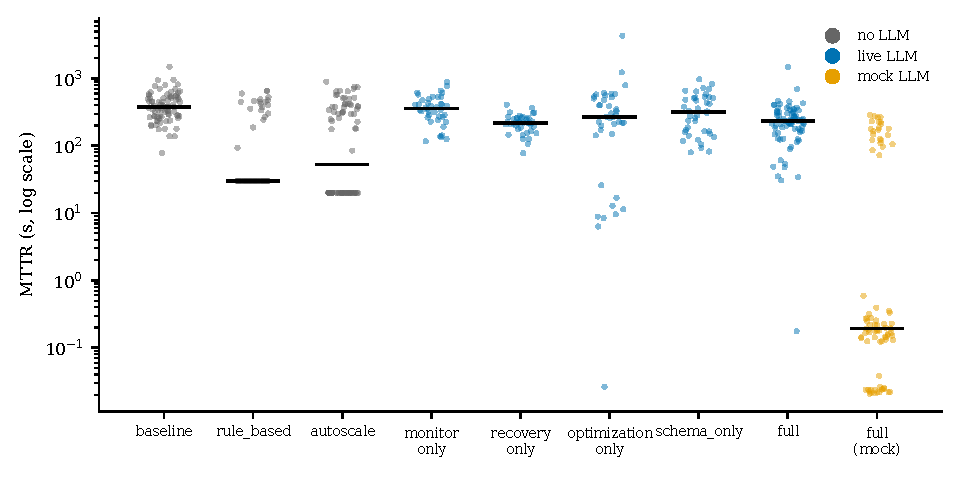
\includegraphics[width=0.75\linewidth]{generated/fig_mttr.pdf}
\caption{Recovery-time distribution by configuration (log scale).}
\label{fig:mttr}
\end{figure*}

\begin{figure*}[t]
\centering
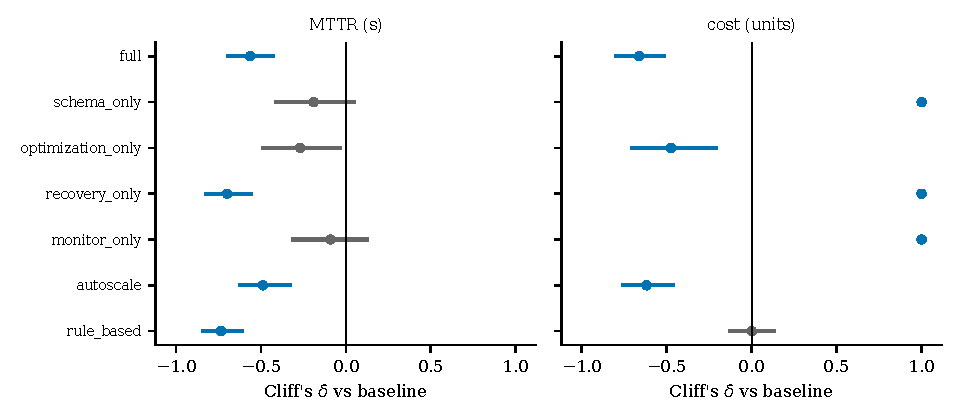
\includegraphics[width=0.95\linewidth]{generated/fig_effects.pdf}
\caption{Cliff's $\delta$ against \texttt{baseline}, by configuration and metric, with bootstrap 95\%
  intervals.}
\label{fig:effects}
\end{figure*}

Table~\ref{tab:main} reports medians with interquartile ranges per configuration, and
Table~\ref{tab:effects} compares each one against \texttt{baseline} using bootstrap confidence
intervals, Cliff's $\delta$, and a Holm-corrected Mann--Whitney $p$-value.
Figures~\ref{fig:mttr} and~\ref{fig:effects} show the underlying distributions and effect sizes. The
\texttt{full} configuration moves MTTR from \NMttrBaselineMedian{}\,s to \NMttrFullMedian{}\,s
($\Delta=\NDiffMttrSFull{}$\,s, $\NRelpctMttrSFull{}$\%, Cliff's $\delta=\NDeltaMttrSFull{}$,
$p_{\mathrm{Holm}}\NPHolmMttrSFull{}$) and cost from \NCostBaselineMedian{} to \NCostFullMedian{}
units ($\NRelpctCostUnitsFull{}$\%, $\delta=\NDeltaCostUnitsFull{}$,
$p_{\mathrm{Holm}}\NPHolmCostUnitsFull{}$). Both effects reach significance, but the MTTR reduction is far
smaller than the mock evaluation of the identical configuration produces
(Section~\ref{sec:livemock}). Cost is the one headline claim that reaches or exceeds the base
paper's reported 25\% reduction, with the caveat, quantified in Section~\ref{sec:sensitivity}, that
it depends on the assumed provisioning gap. The pooled figure also conceals two features of the cost
data. First, the saving is scenario-dependent: \texttt{full}'s median cost sits below
\texttt{baseline}'s in three scenarios but above it in \texttt{ingress\_burst}
(\NCostScenFullIngressBurst{} against \NCostScenBaselineIngressBurst{} units). Second, agent
configurations that skip right-sizing cost far more than \texttt{baseline} in the pooled data:
\texttt{monitor\_only} and \texttt{recovery\_only} by \NRelpctCostUnitsMonitorOnly{}\% and
\NRelpctCostUnitsRecoveryOnly{}\%, and \texttt{schema\_only} by \NRelpctCostUnitsSchemaOnly{}\%. We
did not investigate why. The saving is therefore better attributed to the right-sizing
configurations, chiefly the optimization agent, than to agent control in general.

Manual interventions move in the opposite direction. The median climbs from
\NIntervBaselineMedian{} to \NIntervFullMedian{}
($\Delta=\NDiffManualInterventionsFull{}$, $\NRelpctManualInterventionsFull{}$\%,
$\delta=\NDeltaManualInterventionsFull{}$, $p_{\mathrm{Holm}}\NPHolmManualInterventionsFull{}$), the
reverse of the base paper's reported 70\%-plus reduction, and \texttt{recovery\_only} shows the same
rise ($\NRelpctManualInterventionsRecoveryOnly{}$\%). One plausible mechanism:
\texttt{baseline} escalates exactly once per injected fault by construction, while an agent
configuration that gets rate-limited or budget-denied can propose again on a later tick of the same
300\,s loop, each cycle adding its own escalation. We did not instrument which mechanism dominates,
so we report the measurement and leave the mechanism open (Section~\ref{sec:discussion}). Since
reducing manual interventions is the system's stated purpose, this increase counts as a negative
result for the design, and we report it as one. It answers RQ1: with a live model, the full system
beats static orchestration on recovery time and cost but not on manual interventions.

\subsection{Is the Full System Better Than Cheap, Non-Agent Automation?}

The \texttt{rule\_based} and \texttt{autoscale} configurations call no model and add no cost beyond
the static infrastructure per run, and both still beat every agent configuration on MTTR, including
\texttt{full}. That ranking is conditional on the modelled remediation latencies of
Section~\ref{sec:method}: both comparators resolve covered faults after a fixed 30\,s or 20\,s, so
they reflect what an idealized non-LLM responder could achieve rather than the measured speed of a
deployed one. \texttt{rule\_based} reaches \NMttrRuleBasedMedian{}\,s ($\NRelpctMttrSRuleBased{}$\%
vs.\ baseline, $\delta=\NDeltaMttrSRuleBased{}$) and \texttt{autoscale} reaches
\NMttrAutoscaleMedian{}\,s ($\NRelpctMttrSAutoscale{}$\%, $\delta=\NDeltaMttrSAutoscale{}$), against
$\NRelpctMttrSFull{}$\% for \texttt{full}. Both hold manual interventions flat or drive them down
(\mbox{\NRelpctManualInterventionsRuleBased{}\%} and
\mbox{\NRelpctManualInterventionsAutoscale{}\%}), where \texttt{full} drives them up instead.

On cost, \texttt{autoscale} moves the median by \NRelpctCostUnitsAutoscale{}\%, a smaller cut than
\texttt{full}'s \NRelpctCostUnitsFull{}\%. \texttt{rule\_based}, which does not right-size, shows no
cost effect at all ($\NRelpctCostUnitsRuleBased{}$\%, $p_{\mathrm{Holm}}=\NPHolmCostUnitsRuleBased{}$),
exactly as its design would predict. Neither comparator can execute an accepted mitigation by
construction (\texttt{decision\_correct}$=0$), the one axis on which \texttt{full} wins outright
(Section~\ref{sec:decision}). For these fault scenarios and this control-loop timing, cheap
deterministic automation beats the LLM-driven system on two of four metrics, which answers RQ2 for
idealized comparators: the agent system does not beat cheap automation on speed or on manual
interventions.

\subsection{Decision Quality}\label{sec:decision}

The \texttt{decision\_correct} metric is scored against a per-scenario accepted-mitigation set
(Eq.~\ref{eq:decision}, Section~\ref{sec:method}), and every non-agent configuration scores zero by construction. Among the
agent configurations, only \texttt{full}
($\delta=\NDeltaDecisionCorrectFull{}$, $p_{\mathrm{Holm}}\NPHolmDecisionCorrectFull{}$),
\texttt{optimization\_only} ($\delta=\NDeltaDecisionCorrectOptimizationOnly{}$), and
\texttt{schema\_only} ($\delta=\NDeltaDecisionCorrectSchemaOnly{}$) move the metric significantly;
\texttt{monitor\_only} and \texttt{recovery\_only} do not. Because Cliff's $\delta$ against an
all-zero comparator is algebraically identical to the treatment group's success rate, these values
double as correct-mitigation rates: \texttt{full} executes an accepted mitigation in
$\NDeltaDecisionCorrectFull{}$ of its runs. This is the one metric where the live system achieves
something neither the static baseline nor the rule-based comparator can claim at all, though it only
partly answers RQ3, since fewer than half of the full system's runs act correctly. As
Section~\ref{sec:livemock} shows, the mock evaluation scores the same configuration at
\NLiveVsMockDecisionCorrectMock{}.

\subsection{Per-Scenario Heterogeneity}

\begin{table*}[t]
\centering
\caption{Median MTTR (s) by configuration and scenario.}
\label{tab:scenarios}
\small
\begin{tabular}{lrrrr}
\toprule
config & ingress\_burst & resource\_contention & schema\_drift & upstream\_delay \\
\midrule
baseline & 352 & 386 & 424 & 353 \\
rule\_based & 30.0 & 30.0 & 433 & 30.0 \\
autoscale & 20.0 & 20.0 & 363 & 393 \\
monitor\_only & 366 & 412 & 320 & 275 \\
recovery\_only & 223 & 183 & 224 & 248 \\
optimization\_only & 10.5 & 267 & 502 & 281 \\
schema\_only & 453 & 343 & 120 & 553 \\
full & 148 & 318 & 214 & 237 \\
\bottomrule
\end{tabular}

\end{table*}

\begin{figure*}[t]
\centering
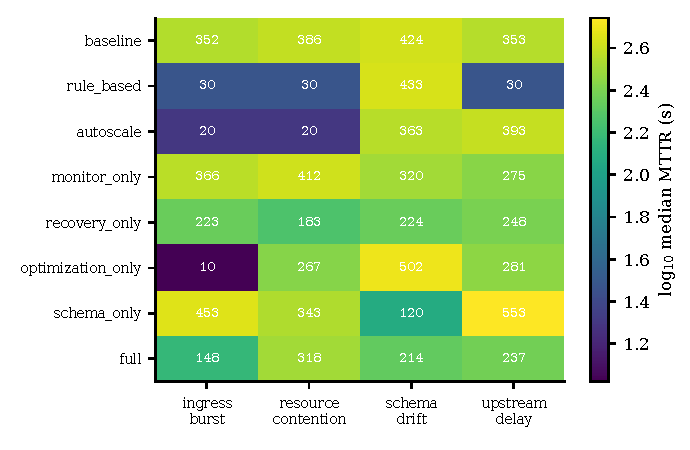
\includegraphics[width=0.85\linewidth]{generated/fig_scenarios.pdf}
\caption{MTTR by configuration and scenario.}
\label{fig:scenarios}
\end{figure*}

Table~\ref{tab:scenarios} and Figure~\ref{fig:scenarios} break MTTR down by (configuration,
scenario). No single configuration dominates every fault type: \texttt{optimization\_only} is
fastest on \texttt{ingress\_burst} but slower than \texttt{baseline} on \texttt{schema\_drift}, a
fault its one enabled non-monitoring agent has no lever on, while \texttt{schema\_only} shows the
mirror pattern. That is the shape a single-agent ablation should take: useful where it owns the
fault, inert or pure overhead everywhere else, which also warns against treating any single
scenario's number as a configuration's typical behavior.

\subsection{Mock Versus Live: The Central Finding}\label{sec:livemock}

\begin{table*}[t]
\centering
\caption{\texttt{full}, live model vs.\ deterministic mock, otherwise identical configuration and
  scenarios; Cliff's $\delta$ with 95\% CI, Holm-corrected $p$.}
\label{tab:live_mock}
\small
\begin{tabular}{lrrrr}
\toprule
metric & live & mock & Cliff's $\delta$ [95\% CI] & $p_{\mathrm{Holm}}$ \\
\midrule
MTTR (s) & 235 & 0.193 & 0.81 [0.72, 0.90] & <0.001 \\
cost (units) & 69.8 & 833 & -0.82 [-0.92, -0.71] & <0.001 \\
manual interv. & 6.00 & 0 & 0.87 [0.79, 0.93] & <0.001 \\
decision correct & 0 & 1.00 & -0.57 [-0.69, -0.46] & <0.001 \\
freshness (s) & 14.0 & 0.0801 & 0.25 [0.074, 0.42] & 0.004 \\
\bottomrule
\end{tabular}

\end{table*}

\begin{figure*}[t]
\centering
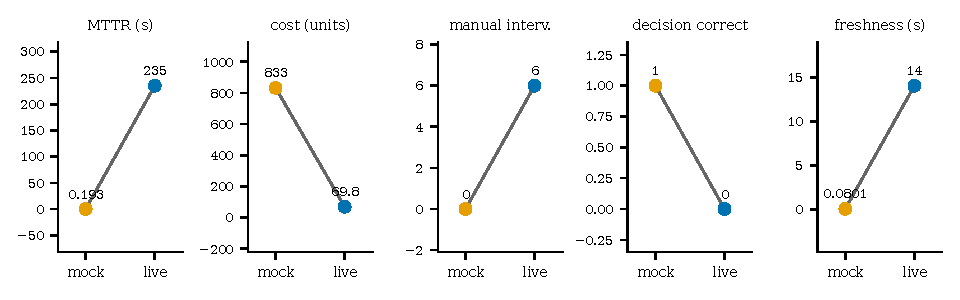
\includegraphics[width=0.95\linewidth]{generated/fig_live_mock.pdf}
\caption{\texttt{full}, live vs.\ mock, per metric (median). Linear axes deliberately: two metrics are
  exactly zero for one arm, which a shared log axis cannot represent.}
\label{fig:live_mock}
\end{figure*}

Table~\ref{tab:live_mock} and Figure~\ref{fig:live_mock} compare \texttt{full} under two conditions
that differ in nothing but the model: arm A (live) against arm C, its deterministic-mock twin. MTTR
drops from \NLiveVsMockMttrSLive{}\,s live to \NLiveVsMockMttrSMock{}\,s mock, a divergence ratio of
$R_{\mathrm{MTTR}}=\NLiveVsMockMttrSRatio{}$ (Eq.~\ref{eq:ratio}); the median decision-correct score
climbs from \NLiveVsMockDecisionCorrectLive{} to \NLiveVsMockDecisionCorrectMock{}, even though the
live correct-mitigation rate is \NDeltaDecisionCorrectFull{}; manual interventions fall from
\NLiveVsMockManualInterventionsLive{} to \NLiveVsMockManualInterventionsMock{}; and freshness falls
from \NLiveVsMockFreshnessSLive{}\,s to \NLiveVsMockFreshnessSMock{}\,s. Cost moves the other way:
live is cheaper than mock (\NLiveVsMockCostUnitsLive{} vs.\ \NLiveVsMockCostUnitsMock{} units), and
the mock's cost even exceeds \texttt{baseline}'s. We did not track down the cause, so this particular
comparison should be read with that caveat attached.

This answers RQ4. The mock evaluation is not a noisier or scaled-down stand-in for the live one; on
recovery time and decision quality it is a categorically different and far more flattering
experiment, and every number earlier in this section should be read with that in mind. The base
paper's headline figures came from some evaluation path, and for one system this campaign measures
just how far that path alone can move the answer. A claim drawn from a mock run about this class of
system is a claim about the mock, not about the model it stands in for.

\subsection{LLM Accounting}

\begin{table*}[t]
\centering
\caption{LLM accounting per agent configuration, counted at the moment a call is or is not made
  (Section~\ref{sec:method}).}
\label{tab:llm}
\small
\begin{tabular}{lrrrrrrr}
\toprule
config & calls & cache hits & degraded & invalid & API tokens & latency (s) & degraded \% \\
\midrule
monitor\_only & 1.00 & 143 & 0 & 0 & 1{,}244 & 4.37 & 0\% \\
recovery\_only & 2.00 & 262 & 0 & 0 & 2{,}737 & 10.5 & 0\% \\
optimization\_only & 2.00 & 258 & 0 & 0 & 2{,}998 & 9.22 & 0\% \\
schema\_only & 2.00 & 274 & 0 & 0 & 2{,}550 & 5.73 & 0\% \\
full & 4.00 & 214 & 0 & 0 & 5{,}946 & 15.0 & 0\% \\
\bottomrule
\end{tabular}

\end{table*}

Table~\ref{tab:llm} reports real model calls, cache hits, degraded proposals, invalid outputs,
tokens, and latency per agent configuration, counted at the moment a call is or is not made
(Section~\ref{sec:method}). Degraded and invalid rates sit at zero across the whole campaign: no run
hit budget exhaustion or a provider outage, and no schema-invalid output survived into the final
runs. That is a property of \emph{this} campaign, not a standing guarantee; the pilot that preceded
it found a live cache-poisoning defect, exactly the kind of failure the accounting exists to catch,
and it was fixed before the campaign began.

The agents' overhead stays small in absolute terms. Across the \NRunsLive{} live-arm runs they made
\NLlmCallsTotal{} real model calls and consumed \NApiTokensTotal{} API tokens in total, and no run
came close to the per-run budget: the largest used \NApiTokensMaxRun{} tokens against a cap of
\NBudgetTokens{}, and at most \NLlmCallsMaxRun{} calls against a cap of \NBudgetCalls{}. The per-run
model latency in Table~\ref{tab:llm} is small next to the 300\,s control loop, so inference time
alone does not explain the live system's recovery time. We do not convert tokens into a monetary
figure, since the provider's per-token prices were never recorded with the runs, leaving token
counts as the portable measure.

\subsection{Sensitivity}\label{sec:sensitivity}

\begin{table*}[t]
\centering
\caption{Closed-form break-even points: the assumed human-latency median (s) and static provisioning
  (units) at which each configuration stops beating its comparator.}
\label{tab:sensitivity}
\small
\begin{tabular}{lrrrr}
\toprule
config & MTTR (s) & human break-even (s) & cost reduction (\%) & static break-even \\
\midrule
autoscale & 52.4 & 49.9 & 47.6 & 3.00 \\
full & 235 & 224 & 55.7 & 2.15 \\
monitor\_only & 359 & 342 & -676 & -- \\
optimization\_only & 267 & 254 & 51.4 & 2.60 \\
recovery\_only & 220 & 209 & -676 & -- \\
rule\_based & 30.0 & 28.5 & 0 & -- \\
schema\_only & 315 & 300 & -484 & -- \\
\bottomrule
\end{tabular}

\end{table*}

\begin{figure*}[t]
\centering
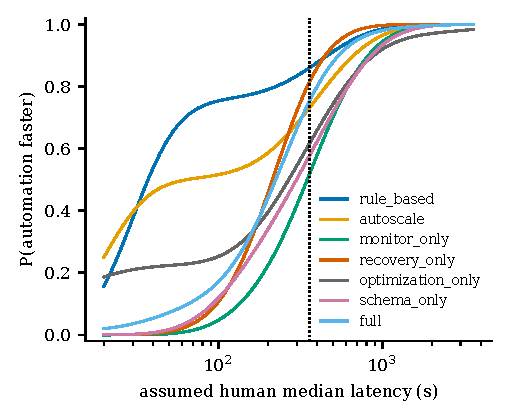
\includegraphics[width=0.75\linewidth]{generated/fig_human_sensitivity.pdf}
\caption{$P(\text{automation faster than the simulated human})$ as a function of the assumed human
  median latency.}
\label{fig:human_sensitivity}
\end{figure*}

\begin{figure*}[t]
\centering
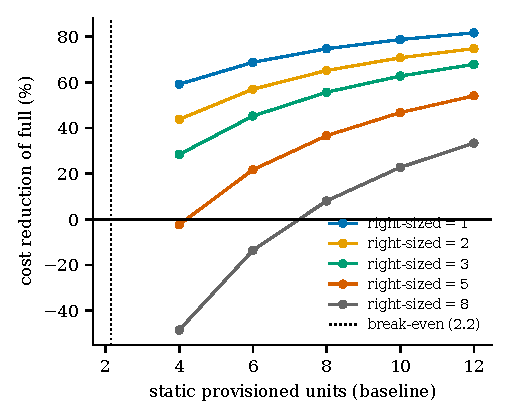
\includegraphics[width=0.75\linewidth]{generated/fig_cost.pdf}
\caption{\texttt{full}'s cost reduction as a function of the assumed static provisioning level.}
\label{fig:cost}
\end{figure*}

Table~\ref{tab:sensitivity} and Figures~\ref{fig:human_sensitivity}--\ref{fig:cost} give the two
closed-form sensitivities from Section~\ref{sec:method}. \texttt{full} keeps beating the simulated
human down to a median latency of \NBreakEvenHumanFull{}\,s, comfortably below the assumed
\NHumanMedian{}\,s yet well above \texttt{rule\_based}'s break-even of
\NBreakEvenHumanRuleBased{}\,s, meaning the rule-based responder's speed advantage tolerates a much
faster on-call than \texttt{full}'s does. On cost, \texttt{full}'s reduction claim survives down to a
static-provisioning assumption of \NBreakEvenStaticFull{} units; below that level, a baseline that
was never badly over-provisioned erases the saving on its own. Both sensitivities drive home the same
point as Section~\ref{sec:livemock} from a different angle: the headline numbers are conditional on
modeling choices, so we report the condition alongside each one.

\subsection{Adversarial Containment}

\begin{table*}[t]
\centering
\caption{Adversarial corpus graded against the independent specification oracle, by category.}
\label{tab:adversarial}
\scriptsize
\begin{tabular}{lrllll}
\toprule
category & cases & containment [Wilson 95\%] & over-block & oracle agreement & fail-open \\
\midrule
boundary\_grid & 4320 & 3056/3056 [0.9987, 1.0000] & 0/1264 [0.0000, 0.0030] & 4320/4320 [0.9991, 1.0000] & 0 \\
defense\_in\_depth & 133 & 133/133 [0.9719, 1.0000] & -- & 133/133 [0.9719, 1.0000] & 0 \\
fuzz & 1000 & 606/606 [0.9937, 1.0000] & 0/394 [0.0000, 0.0097] & 1000/1000 [0.9962, 1.0000] & 0 \\
injection & 28 & 28/28 [0.8794, 1.0000] & -- & 28/28 [0.8794, 1.0000] & 0 \\
param\_extremes & 66 & 44/44 [0.9197, 1.0000] & 0/22 [0.0000, 0.1487] & 66/66 [0.9450, 1.0000] & 0 \\
\textbf{overall} & 5547 & 3867/3867 [0.9990, 1.0000] & 0/1680 [0.0000, 0.0023] & 5547/5547 [0.9993, 1.0000] & 0 \\
\bottomrule
\end{tabular}

\end{table*}

Table~\ref{tab:adversarial} grades the generated corpus (Section~\ref{sec:method}) against the
independent specification oracle, by category and overall, answering RQ5. Overall containment comes
to \NAdversarialContained{}/\NAdversarialUnsafe{} ($\geq\NAdversarialWilsonLo{}$, Wilson 95\%). The
over-block rate on legal, non-unsafe proposals is zero, with the exact denominator given in the
table. The policy agrees with the oracle on all \NAdversarialCases{}/\NAdversarialCases{} graded
cases, with \NAdversarialGateErrors{} gate errors. These figures were measured \emph{after} the two
contract-layer fixes, L6(i)--(ii), that an earlier pass of the same corpus forced
(Section~\ref{sec:lessons}); they describe the fixed system, and the corpus that exposed the gaps now
serves as a committed regression test against exactly this claim.
